\documentclass[11pt, letterpaper,titlepage]{article}

% --- Essential Packages ---
\usepackage[utf8]{inputenc}
\usepackage[margin=1in]{geometry}
\usepackage{fancyhdr} % For custom headers and footers
\usepackage{graphicx}
\usepackage{amsfonts}

\usepackage{amsmath}
\usepackage{float}

\usepackage{hyperref}
\usepackage{setspace}

% --- Header/Footer Configuration ---
\pagestyle{fancy}
\fancyhf{} % Clear all default header and footer settings
\fancyhead[L]{NOTES EECE 5644} % Left header text
\fancyhead[C]{} % Center header text (empty)
\fancyhead[R]{\thepage} % Right header (page number)
\renewcommand{\headrulewidth}{0.4pt} % Line below header
\linespread{1.2}






\begin{document}
\begin{titlepage}
    \centering
    \vspace*{0cm}
    
    {\Huge \textbf{Speech Noise Reduction Using Long \\ \vspace{0.5cm}Short-Term Memory Neural Networks}} \\[1cm]
    
    \vspace{4cm}
    
    \textit{\textbf{Abstract:} }
    
    \vspace{4cm}
    {\Large \textbf{Skylar Denno}}
    

    
    \vspace{0.8cm}

    
    Department of Electrical and Computer Engineering \\
    Northeastern University \\
    \vspace{0.8cm}
    
    
    \today
    
        \vspace{0.8cm}
        
        \textbf{GitHub:} \textit{https://github.com/skylar-slideshows/ML\_denoise}
    
\end{titlepage}

\section{Introduction}



\subsection{Problem Definition}

Speech recordings often contain unwanted background noise from sources such as traffic, conversations, wind, or electronic interference. This noise reduces speech quality and intelligibility, making communication more difficult for human listeners and automatic speech recognition systems. Traditional signal processing methods can reduce some types of noise, but they usually rely on fixed assumptions about the noise characteristics and often perform poorly when the noise changes over time.

Machine learning provides an alternative by learning the relationship between noisy and clean speech from examples. By chopping incoming audio into short frames and using machine learning to predict the spectral characteristics of the clean audio for that frame based on actions during previous frames, the system will be able to deal with highly dynamic, complex noise such as other people talking in the background or music in the background.

\subsection{Dataset Definition and EDA}

The dataset used was the "Noisy speech database for training and speech enhancement algorithms" from the University of Edinburgh's DataShare program. Specifically, the 28 speaker trainset (separated into clean and noisy pairs) was to be used. The model would be trained to learn the "difference" between the noisy recording and its corresponding clean recording, and it would later use that training to infer the difference for new audio. A set of test pairs were also provided, with no speaker appearing in both the test and training sets.

\noindent \textbf{Dataset Name:} Noisy speech database for training speech enhancement algorithms and TTS models

\noindent \textbf{Dataset Source:} University of Edinburgh: DataShare, School of Informatics, Centre for Speech Technology Research (CSTR)

\noindent \textbf{Dataset Link:} https://doi.org/10.7488/ds/2117 

\noindent \textbf{Number of Files:} 11,572 (pairs of audio files: one clean, one with noise)

\noindent \textbf{Number of Samples:} The total number of short-time Fourier transform (STFT) frames across all the audio files. Each frame is 512 audio samples long (32ms each at the training sample rate of 16kHz).

\noindent \textbf{Target:} Parameters (values on each of the 257 frequency bins for the spectral mask to filter out) per frame of audio.
 

\section{Data Preprocessing}

\subsection{Cleaning}

The dataset provided by The University of Edinburgh is already well organized and does not appear to include any problem data. However, a dedicated cleaning and data validation script was written to ensure that all the data we would use would work for our specific machine learning model and implementation. Additionally, if using other datasets for future training, the cleaning script will be able to validate and filter files for those datasets too.

The preprocessing script checked that each clean speech file had a matching noisy speech file. To test, I temporarily removed 8 of the audio files from the clean folder, but not the noisy folder. Upon running the preprocessing script, this was the output:


\begin{figure}[H]
    \centering
    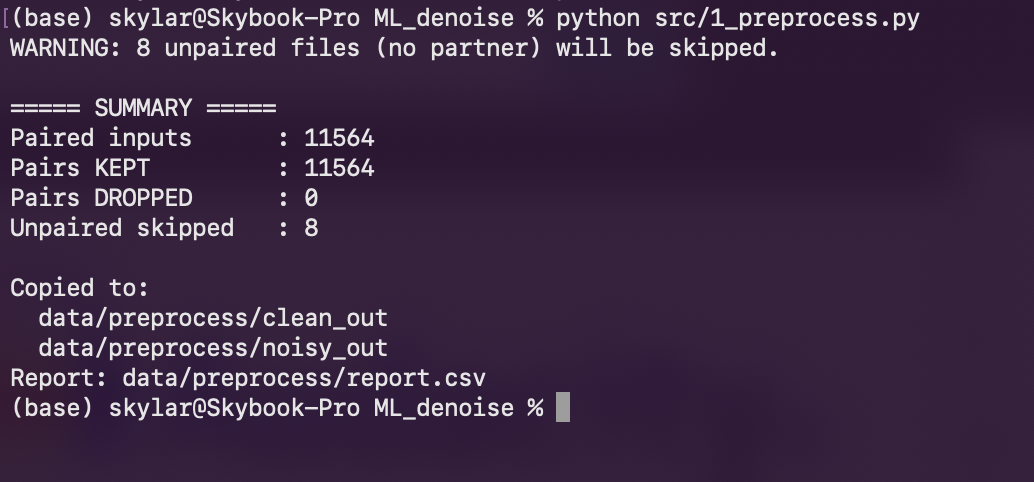
\includegraphics[width=0.6\textwidth]{unpaired.png}
    \caption{Preprocessing script output after severing 8 pairs}
\end{figure}

All the files, except ones without partners, were copied to a new preprocessed data folder.

Next, any silent audio files (containing no samples louder than -40dBFS (decibels full scale) were to be removed. To test this, I added two silent audio files each, with the same names, to the clean and noisy folders and ran the script:

\begin{figure}[H]
    \centering
    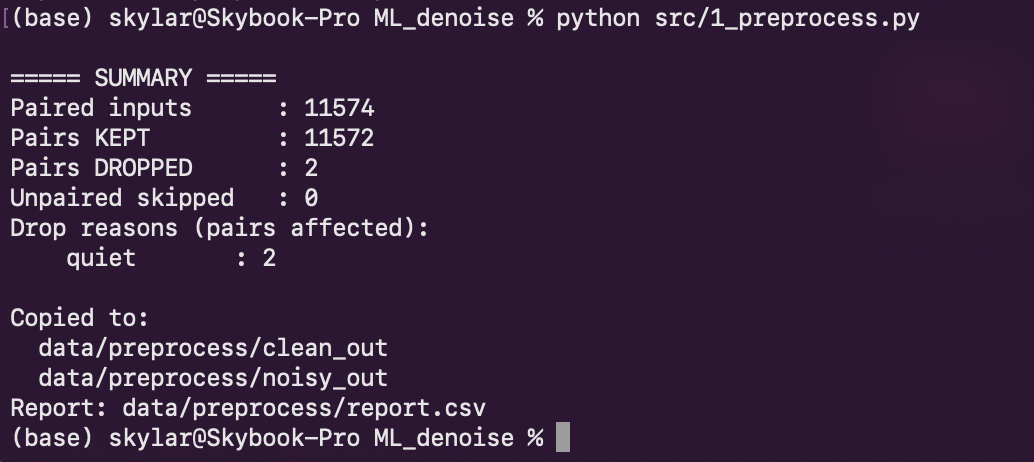
\includegraphics[width=0.6\textwidth]{silence.png}
    \caption{Preprocessing script output after adding 2 pairs containing silence}
\end{figure}

\begin{figure}[H]
    \centering
    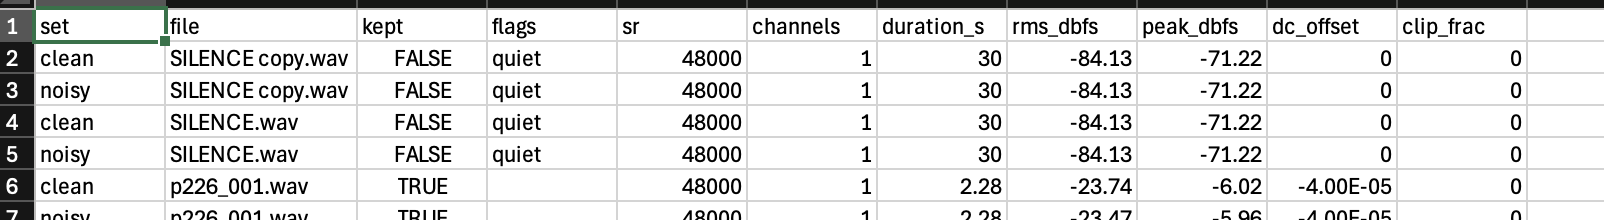
\includegraphics[width=0.6\textwidth]{silence2.png}
    \caption{Preprocessing script report.csv after adding 2 pairs containing silence}
\end{figure}

The report.csv output showed the 2 pairs that were not copied to the preprocessed data folder. The reason is given as "quiet."

Next, for very loud signals (where a large proportion of audio samples are near the maximum amplitudes at -1 and 1), we want to remove them, as this digital clipping, or shaving off of the peaks of the waves, causes distortion and will be bad to train the model on. I placed two identical files of full-scale square wave at 440Hz (containing samples only at -1 and 1) in the clean and noisy folders. I ran the preprocessing script:

\begin{figure}[H]
    \centering
    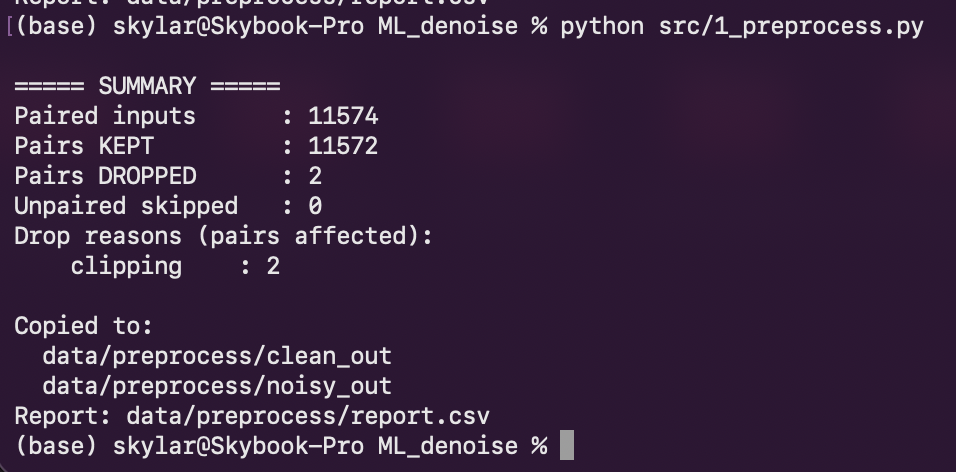
\includegraphics[width=0.6\textwidth]{clip.png}
    \caption{Preprocessing script output after adding 2 pairs containing clipping}
\end{figure}

\begin{figure}[H]
    \centering
    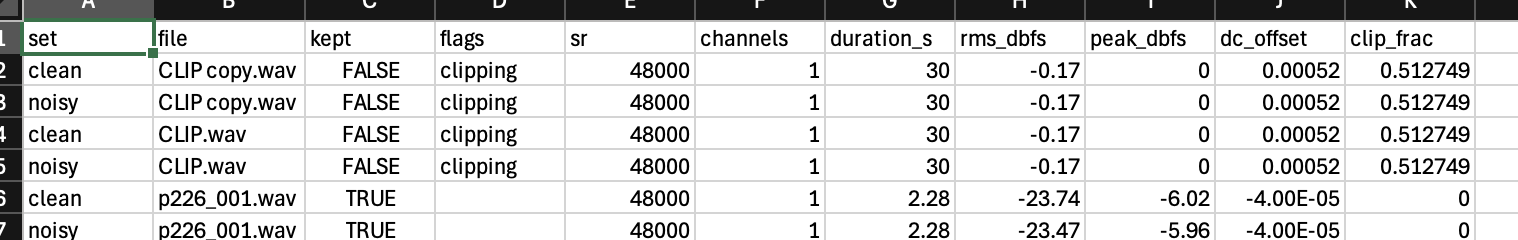
\includegraphics[width=0.6\textwidth]{clip2.png}
    \caption{Preprocessing script report.csv after adding 2 pairs containing clipping}
\end{figure}

The script similarly detected and flagged these files, keeping them out of the preprocessed data folder.

After this, I created two audio files containing white noise at a medium volume (to not trigger clipping or silence flags), but with durations of 163ms (below the 1s minimum length threshold). I also accidentally exported these files with a 44.1kHz sample rate, which also caused the bad\_sr flag. It is important for the sample rates to all be consistent, since a discrete Fourier transform was to be used.

\begin{figure}[H]
    \centering
    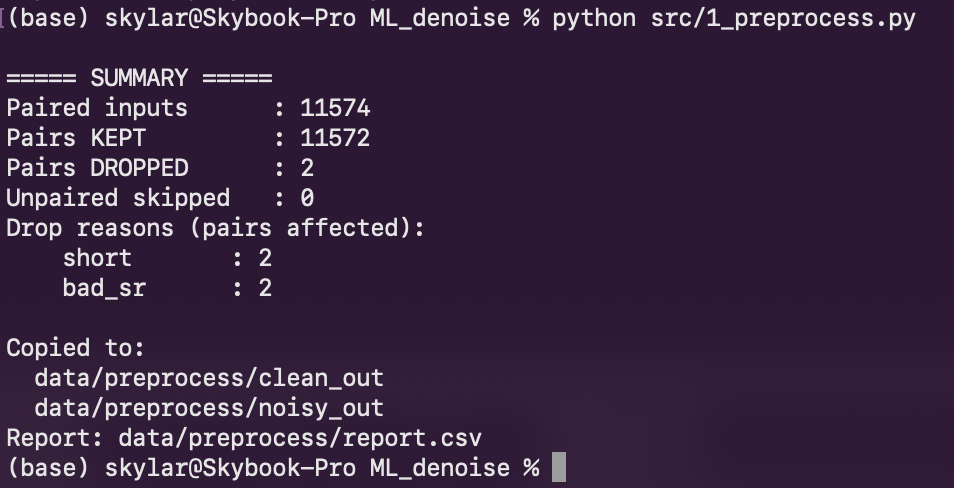
\includegraphics[width=0.6\textwidth]{short.png}
    \caption{Preprocessing script report.csv after adding 2 pairs of very short audio (44.1kHz)}
\end{figure}

\begin{figure}[H]
    \centering
    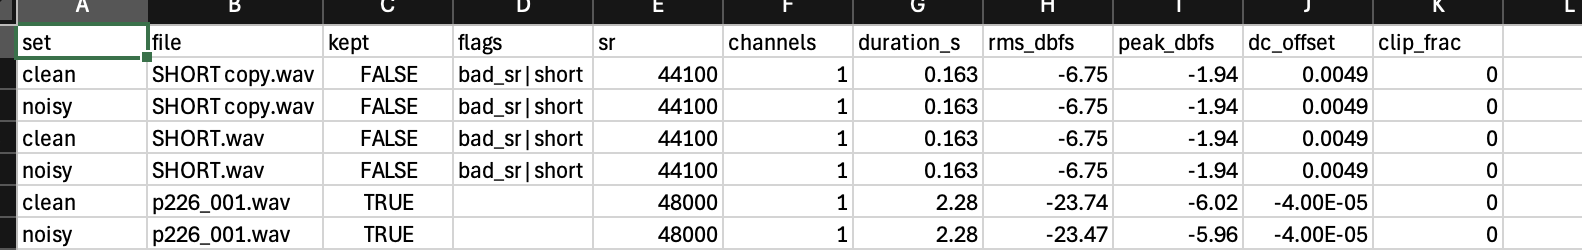
\includegraphics[width=0.6\textwidth]{short2.png}
    \caption{Preprocessing script report.csv after adding 2 pairs of very short audio (44.1kHz)}
\end{figure}

The script similarly detected and flagged these files, keeping them out of the preprocessed data folder.

Additionally, (but not shown) the script checked for files with a DC offset (the mean value of all the samples is significantly different than 0; the audio is not symmetrical about 0).

A CSV report recorded the results for each file to provide a complete quality control summary. Files that failed any required validation check were to be excluded automatically. However, since the University of Edinburgh noisy speech dataset is well curated and consistently labeled, all file pairs passed the validation checks, as expected. No files were removed from the dataset.

\begin{figure}[H]
    \centering
    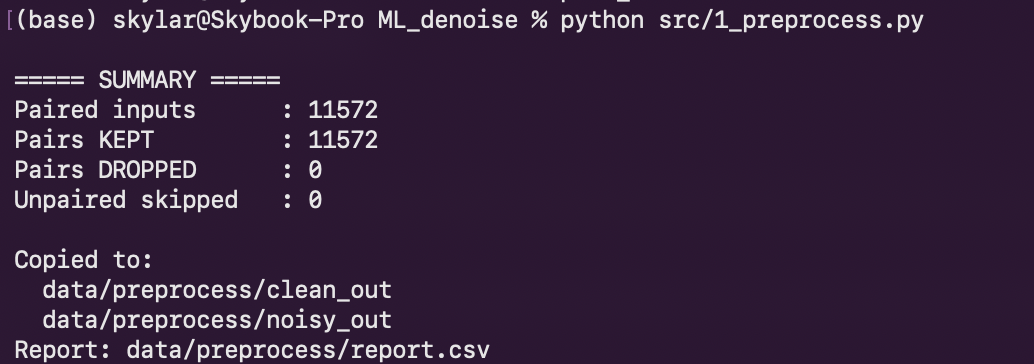
\includegraphics[width=0.6\textwidth]{ideal.png}
    \caption{Preprocessing script output for the actual dataset.}
\end{figure}

To make my end product as easy to use and reproduce as possible, I included individual config files for each of the scripts in the project folder. In the preprocessing config, the thresholds to filter good and bad files can be easily changed, as well as the file paths for the data input and output folders.

\begin{figure}[H]
    \centering
    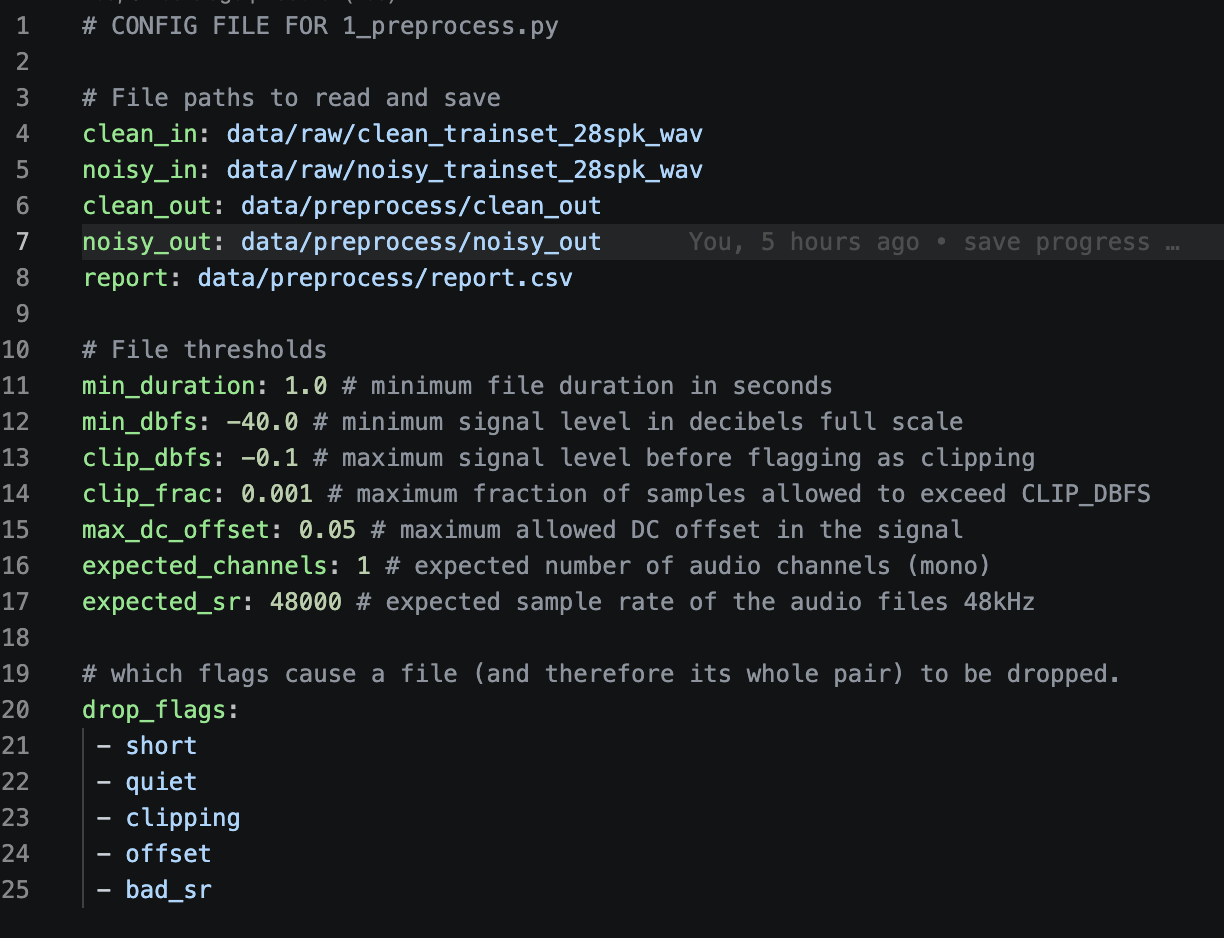
\includegraphics[width=0.7\textwidth]{config.png}
    \caption{1\_preprocess.yaml Config file}
\end{figure}

\subsection{Encoding, Feature Engineering, and the Short-Time Fourier Transform}

The training model will not be taking in the array of signal sample values directly from the audio file, but instead, a set of complex values of the Fourier transform of each audio file. This is because the noise masking problem is inherently frequency based, so a Fourier transformed set of data makes much more sense for this application. However, the problem is also time based, since the noise changes over time, and a single fixed mask would not be sufficient, so we are not using a regular Fourier transform. Instead we are using a short time Fourier transform (STFT), which breaks the signal up into small frames, before applying the transform to each frame separately.

Therefore, a script "2\_encode.py" was created to take in the preprocessed sound files (separated into clean and noisy folders) and create corresponding STFT arrays for each file. The arrays would contain as many columns are there are frequency bins for each frame of audio, and as many rows as there are frames for that specific file. 

\begin{figure}[H]
    \centering
    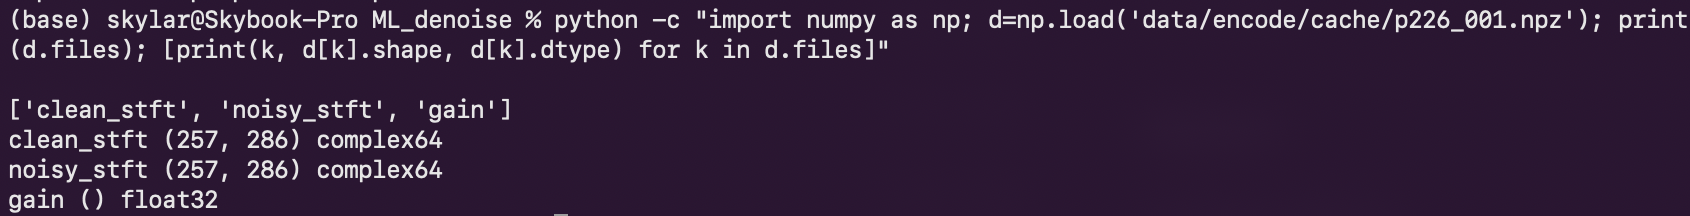
\includegraphics[width=0.8\textwidth]{encode.png}
    \caption{Checking the array shape of one of the encoded data files. The first dimension (257) is the number of frequency bins across the audio spectrum that the audio is divided into (257 complex numbers). The second dimension is the number of time frames that the audio was split into. Each time frame for this training run, at 16kHz sample rate. was 512 samples (about 32ms). For this particular file, there are 286 time frames, meaning the file was about 9 seconds long.}
\end{figure}


\subsection{Training and Validation Split}

After encoding, a make\_split script was written to assign some of the speakers to a validation/test set, and the rest to the training set. I made the decision to split at the speaker level, rather than the individual file level. In other words, no recordings of the same person person will appear in both the training and validation sets. This prevents the model from learning from the specific qualities of the speakers' voices, which would make the testing look better than it would actually perform in genuine trials, where none of the model's training set speakers match the real-life speaker's exact vocal characteristics. 

\begin{figure}[H]
    \centering
    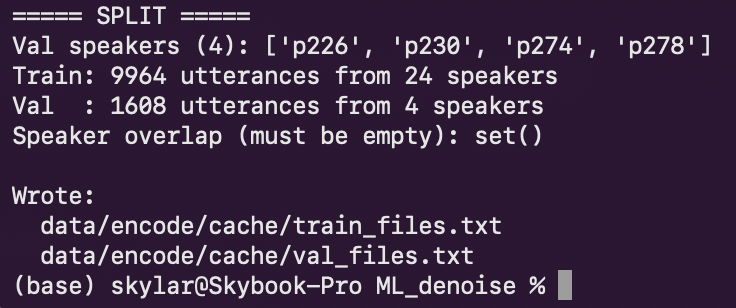
\includegraphics[width=0.5\textwidth]{split.png}
    \caption{3\_make\_split.py script output. This script uses a seed (set in its config file) to ensure reproducability. For now, we are defaulting to a ratio of 4 validation speakers, 24 training speakers}
\end{figure}

The file names for each set are written to separate text documents, and the ML training script just needs to use the corresponding files, located in the encoding folder, containing the STFT arrays.

The data is now ready to be used in the training process.


\section{Machine Learning}

\subsection{Model Selection}

Noise in recordings changes over time dynamically, but between single frames (32ms), the spectral characteristics of the noise is likely to be similar. It is easier to predict what the spectral mask should be for the next frame if you know what it was for the previous one. Therefore, this kind of noise processing is heavily context and sequence dependent, so it was natural to use a recursive neural network. Recursive Neural Networks (RNNs) are often used for audio problems like this, where the data is temporal and sequential, therefore requiring a model with "memory" of past inputs.

Next, we want to pick a specific RNN variant, since RNNs cover a vast range of different models. For this project, a long-short term memory network is chosen (LSTM). This is because of the nature of the data we are using. Each individual speech clip may be several seconds long, but each unit for time recursion: individual audio frames of 32ms / 512 samples are very short. There will be hundreds per file, so when the model needs to figure out the relationship between the current frame and the past hundreds of frames, the problem of vanishing gradients will become significant. If hundreds of gradient values (usually less than 1) are multiplied together during back propagation, the resulting gradient will be nearly 0, and the model will not be able to "understand" the relationship between the current frame and much earlier frames of audio.

Since LSTMs use cell states which additively combines previous gradients, rather than multiplicatively, they are the best choice for a problem like this, where we will often need context from hundreds of frames and gradients in the past. I plan to use the Python PyTorch "torch.nn.lstm" class to implement this model.

This model will be used under the "many-to-many" framework, as each trial will take in numerous frames of audio from an audio file and output numerous frames of complex values (257 per frame) to reconstruct what the model "thinks" the denoised audio spectrum should be, using DSP.


\subsection{Model Evaluation and Performance Metrics}
Validation loss and Mean Squared Error (MSE) were used as the primary regression metrics because the model predicts continuous-valued spectrogram magnitudes rather than discrete classes. Validation loss measures the average reconstruction error on speech recordings that were not used to update the model weights, providing an indication of how well the network generalizes to unseen data. MSE similarly measures the average squared difference between the predicted and target spectrogram magnitudes, with lower values indicating more accurate reconstruction. Together, these metrics provide a direct measure of the model's learning progress and are used to compare different model configurations during training and hyperparameter tuning.



However, there is still the question of how we will evaluate the model's performance quantitatively, with respect to the actual quality of the output audio, since just "listening" to the test output and saying it sounds less noisy or more intelligible is not enough. Therefore, in addition to standard we will evaluate denoising performance using three standard objective metrics, each capturing a different aspect of speech quality.

\subsubsection*{PESQ (Perceptual Evaluation of Speech Quality)}
PESQ estimates the perceptual quality of the enhanced speech,
i.e.\ how natural and pleasant it sounds to a human listener. It
compares the enhanced signal against the clean reference using a model
of human auditory perception, accounting for how the ear responds to
different frequencies and loudness levels. PESQ scores typically range
from -0.5 to 4.5, where higher values indicate better perceived
quality. Because it models perception rather than raw signal error,
PESQ correlates reasonably well with human opinion scores.

\subsubsection*{STOI (Short-Time Objective Intelligibility)}
STOI measures intelligibility (how understandable the speech
is) which is distinct from how pleasant it sounds. It compares the
short-time temporal envelopes of the enhanced and clean signals across
frequency bands, since intelligibility depends largely on preserving
these envelope patterns. STOI produces a score between 0 and 1
(often reported as a percentage), where higher values indicate more
intelligible speech. A signal can sound distorted yet remain highly
intelligible, so STOI captures information that PESQ does not. We don't want each filter mask to be very different from frame to frame, producing a garbled, highly varying output that is hard to understand.

\subsubsection*{SI-SDR (Scale-Invariant Signal-to-Distortion Ratio)}
SI-SDR measures raw signal fidelity (how close the enhanced
waveform is to the clean reference) expressed in decibels. It
decomposes the estimate into a component aligned with the target and a
residual distortion component, and reports their ratio. The
scale-invariant property means the metric is unaffected by overall
amplitude scaling, so it rewards correct signal shape rather
than matching loudness. Higher values (in dB) indicate less
distortion. Unlike PESQ and STOI, SI-SDR is a purely mathematical
measure and does not model human perception.

\subsubsection{Why Use All Three}
The three metrics capture complementary aspects: PESQ reflects
perceptual quality, STOI reflects intelligibility, and SI-SDR reflects
signal fidelity. A model may improve one while degrading another. For
example, aggressive noise suppression can raise SI-SDR while
introducing artifacts that lower PESQ. Reporting all three provides a
more complete picture of denoising performance than any single metric
alone.

\subsection{Training}


The speech denoising model was trained using supervised learning on paired noisy and clean speech recordings that had already been validated, encoded, and divided into training and validation sets. Each training sample consisted of the log-magnitude spectrogram of a noisy speech recording as the model input, while the corresponding clean magnitude spectrogram served as the target output. Working in the frequency domain allows the model to learn how background noise affects different frequency components of speech, rather than attempting to predict waveform samples directly.

Because the speech recordings vary in duration, the resulting spectrogram sequences also vary in length. Mini-batches therefore cannot be formed by simply stacking the input tensors. During data loading, each sequence in a batch is padded to the length of the longest sequence, while the true sequence lengths are recorded. These lengths are then used with PyTorch's sequence packing utilities so that the LSTM processes only valid speech frames rather than the padded values. During loss computation, a masked Mean Squared Error (MSE) function ignores all padded frames, ensuring that only genuine speech data contributes to the optimization process. This approach allows efficient mini-batch training without introducing errors from artificial padding.

The network architecture consists of a bidirectional Long Short-Term Memory (LSTM) network followed by a fully connected output layer. For every time frame, the model predicts a frequency-dependent gain that is applied to the noisy magnitude spectrogram to estimate the corresponding clean speech spectrogram. Since speech characteristics evolve over time, the recurrent structure enables the model to use temporal context from surrounding frames instead of processing every frame independently. This improves the continuity of the enhanced speech and allows the model to distinguish speech from background noise more effectively.

Training was performed using the Adam optimization algorithm with mini-batch gradient descent. After each training epoch, the model was evaluated on a separate validation set containing speakers that were not included in the training set. This speaker-level separation provides a more realistic measure of generalization because the model must denoise voices that it has never encountered during training. A checkpoint was saved after every epoch, while the checkpoint with the best validation performance was also saved separately for later inference. Selecting the model according to validation performance helps reduce overfitting and ensures that the final network represents the best-performing training state rather than simply the final epoch. During training, several performance metrics, including validation loss, Mean Squared Error (MSE), coefficient of determination (R²), accuracy, F1-score, and ROC-AUC, were reported to monitor convergence and model behavior throughout the optimization process.

For the first training run, the decision was made to make the model only use past frames in its inference, and not future frames (unidirectional LSTM). The sample rate was also set to 16kHz which would only cover the important parts of the hearing range for speech. This is simpler and more practical, as it can be used in live/real-time processing, such as conference call software, where future data is not known. This version would be likely to be used in such applications, where speed and real-time processing was the goal. A second training run was later performed to attempt to get the best possible quality and results. The LSTM was set to bidirectional (using both future and past frames), and the sample rate was increased to 44.1kHz (a standard rate for audio recordings that covers the entire hearing spectrum). The first run used 25 epochs, with a batch size of 4. The second (high-quality audio) training run used 32 epochs, with a batch size of 8. The number of samples per frame of audio during encoding was also increased from 512 to 2048, to maintain a similarly time-length window size despite the faster sample rate.

\subsection{Hyperparameter Tuning}



The performance of an LSTM network depends strongly on its hyperparameter values. Parameters such as the hidden layer size, number of recurrent layers, learning rate, dropout probability, and weight decay determine both the learning dynamics and the model's ability to generalize to unseen data. Selecting these values manually is often inefficient and may result in suboptimal performance. Therefore, an automated hyperparameter tuning framework was developed to evaluate multiple candidate configurations systematically.

The tuning procedure uses a grid search strategy. Candidate values for each hyperparameter are specified in the configuration file, and the training software automatically generates combinations of these values. Each candidate model is trained for a reduced number of epochs using the same training and validation data splits as the full training process. Limiting the number of epochs allows many configurations to be evaluated within a practical amount of time while still providing a reliable indication of their relative performance.

After each trial, the selected objective metric is evaluated on the validation set. By default, the tuning process minimizes the validation Mean Squared Error (MSE), although the software also supports selecting alternative optimization objectives such as R², accuracy, F1-score, or ROC-AUC. The configuration that achieves the best validation performance is recorded along with its associated hyperparameter values and training statistics. A summary of every trial is written to an output file so that the complete search process can be reproduced and analyzed later.

Once the search process identifies the best-performing configuration, the model can optionally be retrained using those hyperparameters and the complete training schedule. This two-stage procedure reduces the computational cost of hyperparameter optimization while allowing the final model to benefit from both systematic parameter selection and a full training run. Compared with manual trial-and-error, this approach provides a more objective method for selecting model parameters and improves the likelihood of obtaining a network that generalizes well to previously unseen speakers and recording conditions.




\subsection{Results}

The training was run locally, (on capable hardware), due to the need for convenient parameter editing, reruns, and the very large dataset. Training showed a characteristic quick improvement early on and gradual improvement in later epochs, with occasional epochs not performing better than the previous. All checkpoint files, from every epoch, were saved to the GitHub repository. Any epoch's model can be run on by editing the path in 5_infer.yaml or 5_infer_BATCH.yaml config files to point to the desired PyTorch .pt artifact file in the artifacts folder. The first few epochs produced very garbled, watery sounding audio which was completely unintelligible. In subsequent epochs, the audio became more intelligible, and all metrics (including the audio-specific ones) approached more ideal values. By the last ten epochs, the output audio was almost always more intelligible than the noisy input, and only subtle improvements were being made.

Both the 16kHz standard quality run and the 44.1kHz high quality run produced final models that performed very well with ROCAUC values >= 0.99995, MSE <= $10^{-6}$, and loss <= $4*10^{-4}$. Qualitatively, the output audio was very clear, and it was surprising how much detail in the voice recordings were revealed, that had been previously masked by noise, especially in the high-quality model.

All of the learning curves shown below are from the standard, 16kHz real-time capable (unidirectional LSTM) run. I believe this is likely to be the more practical model in real-life use, unless high quality, post-processing audio recovery is needed.

\begin{figure}[H]
    \centering
    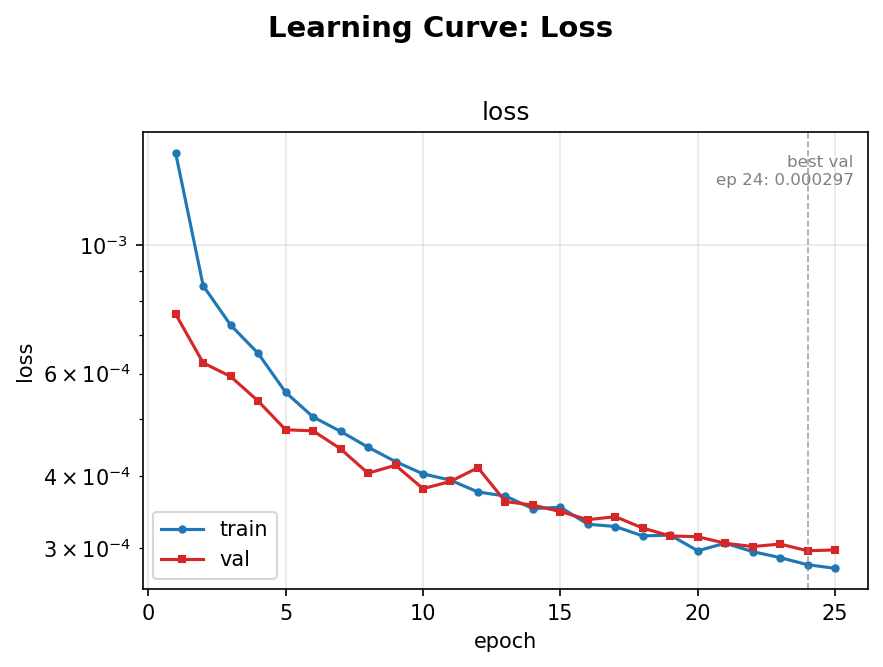
\includegraphics[width=0.6\textwidth]{loss.png}
    \caption{Learning curves on training/validation loss}
\end{figure}

\begin{figure}[H]
    \centering
    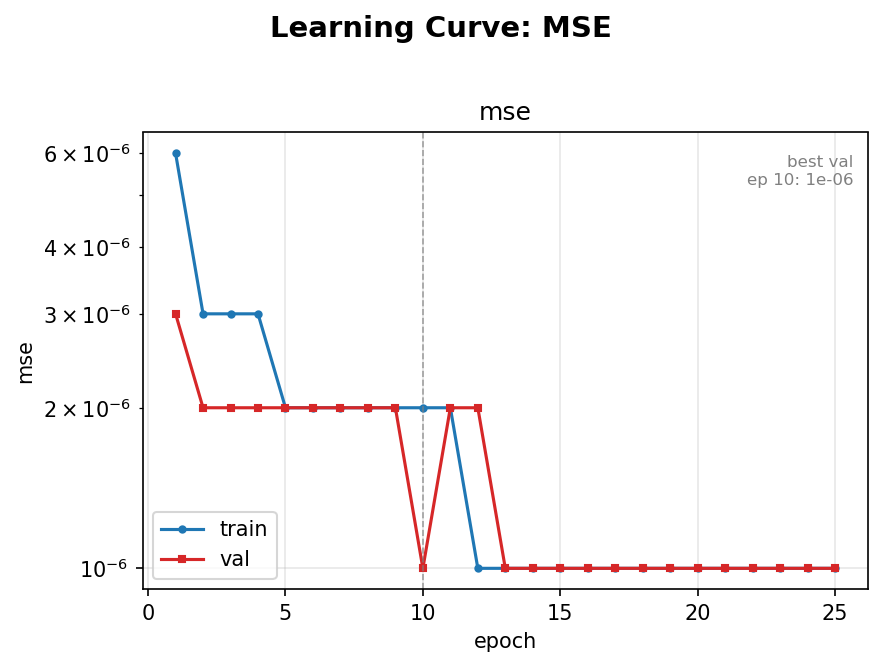
\includegraphics[width=0.6\textwidth]{mse.png}
    \caption{Learning curves on Mean Standard Error (MSE)}
\end{figure}

\begin{figure}[H]
    \centering
    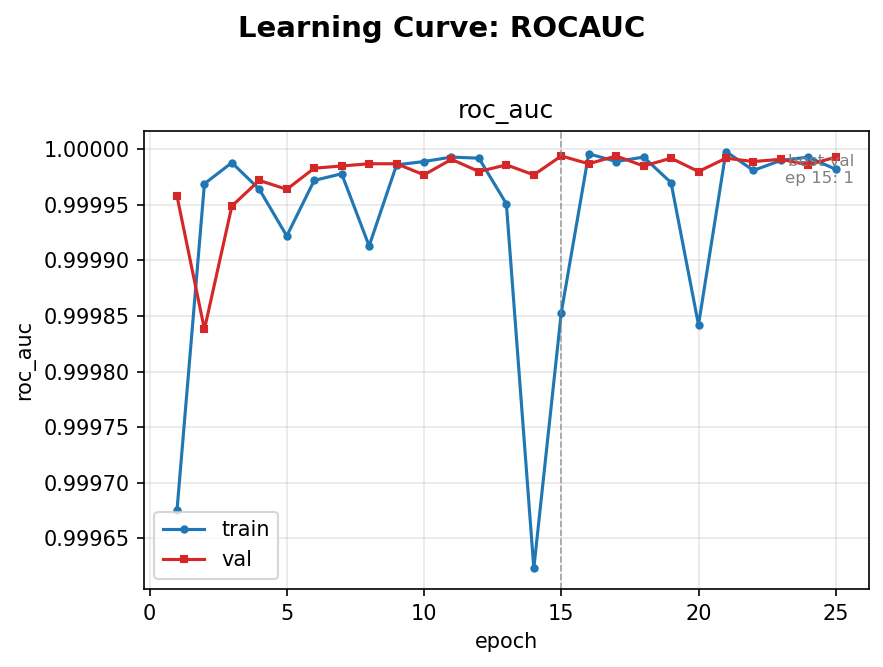
\includegraphics[width=0.6\textwidth]{roc_auc.png}
    \caption{Receiver Operating Characteristic Area Under the Curve (ROCAUC) learning curve. a score of 1 signifies the model perfectly predicts the denoised audio from the noisy input. We see the numbers are very close to this with a very very slight upward trend, after the first five epochs.}
\end{figure}

\begin{figure}[H]
    \centering
    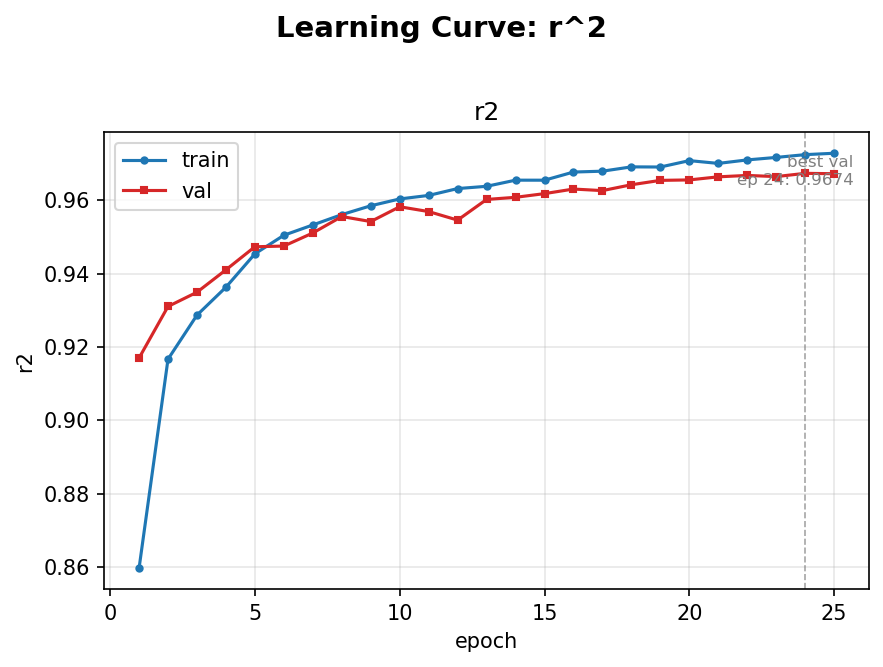
\includegraphics[width=0.6\textwidth]{r2.png}
    \caption{$R^2$ learning curve}
\end{figure}

\begin{figure}[H]
    \centering
    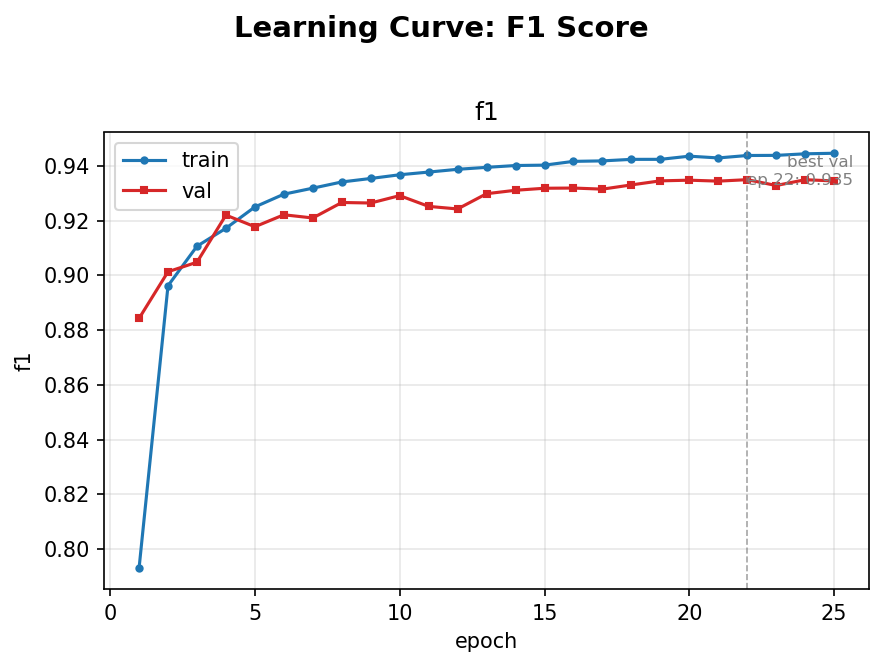
\includegraphics[width=0.6\textwidth]{f1.png}
    \caption{F1 Score learning curve}
\end{figure}

Below are the confusion matrices of the best final epochs of each run. First, the high-quality 44.1kHz run, and then the 16kHz run.

\begin{figure}[H]
    \centering
    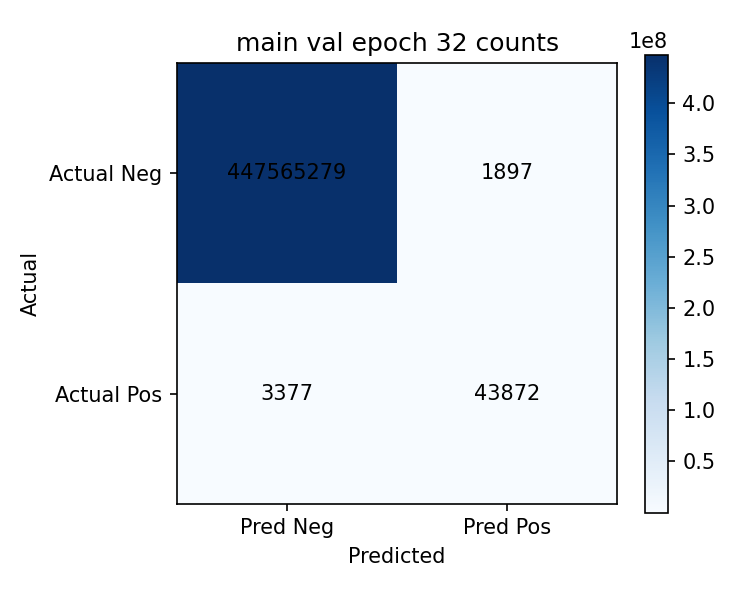
\includegraphics[width=0.6\textwidth]{main_val_epoch_032_counts.png}
\end{figure}

\begin{figure}[H]
    \centering
    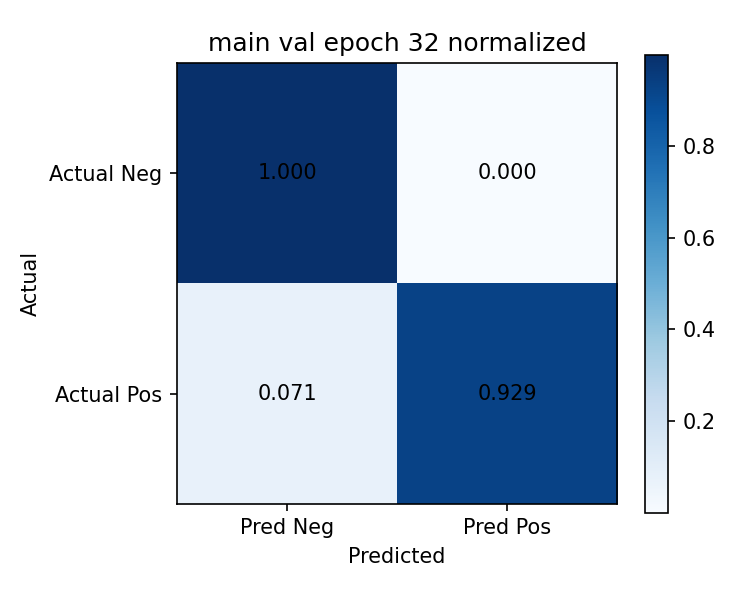
\includegraphics[width=0.6\textwidth]{main_val_epoch_032_normalized.png}
\end{figure}

\begin{figure}[H]
    \centering
    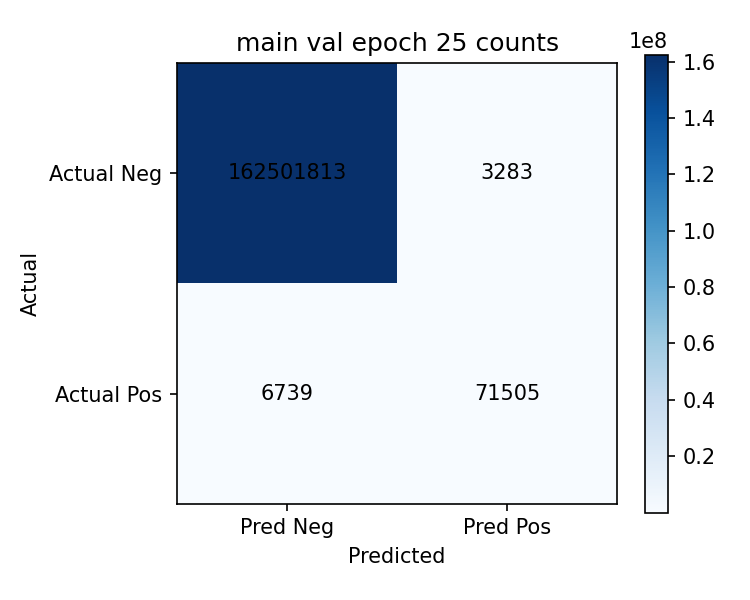
\includegraphics[width=0.6\textwidth]{main_val_epoch_025_counts.png}
\end{figure}

\begin{figure}[H]
    \centering
    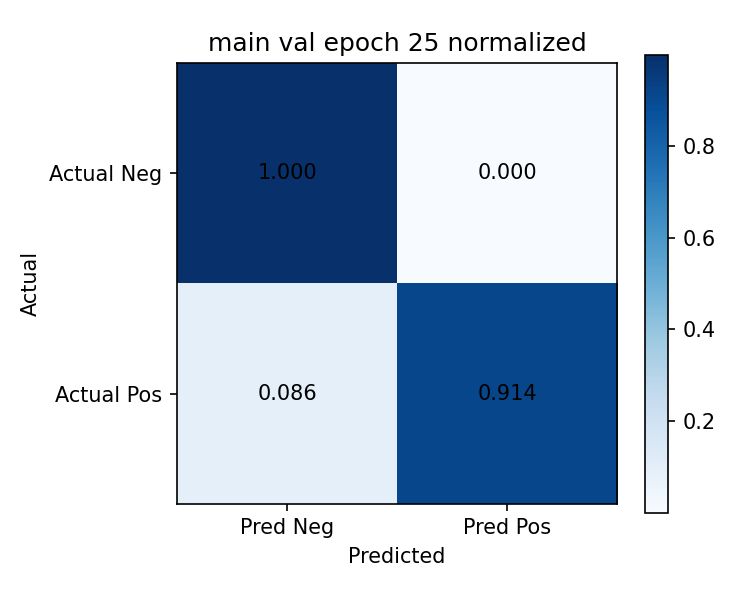
\includegraphics[width=0.6\textwidth]{main_val_epoch_025_normalized.png}
\end{figure}


\section{Discussion}

The results of this project demonstrate that Long Short-Term Memory (LSTM) networks are well suited to the task of speech enhancement. By processing speech as a sequence of short-time Fourier transform (STFT) frames rather than independent samples, the network was able to exploit the temporal structure of speech and distinguish it from background noise. As training progressed, both the objective evaluation metrics and subjective listening tests showed consistent improvement, indicating that the model successfully learned the relationship between noisy and clean speech recordings.

One of the most important design decisions was to split the dataset at the speaker level rather than at the individual recording level. This ensured that the validation set contained speakers that the model had never encountered during training, providing a more realistic measure of generalization. The consistently low validation loss and Mean Squared Error (MSE) suggest that the model did not simply memorize characteristics of the training speakers, but instead learned features of speech and noise that transferred to previously unseen voices.

The comparison between the two training configurations also highlighted the trade-off between reconstruction quality and practical deployment. The unidirectional LSTM operating at 16~kHz produced high-quality speech while remaining suitable for real-time applications, since only past audio frames are required during inference. In contrast, the bidirectional 44.1~kHz model achieved the highest overall speech quality by incorporating both past and future context, but this improvement comes at the cost of increased computational requirements and the inability to perform causal, real-time processing. The choice between these models therefore depends on the intended application, with live communication systems favouring the former and offline speech restoration benefiting from the latter.

The automated preprocessing and validation pipeline also proved valuable, even though the University of Edinburgh dataset required no cleaning in practice. The validation scripts verified file pairing, sample rate, recording duration, clipping, silence, and other quality measures before feature extraction began. While all files in the dataset passed these checks, the testing performed with deliberately corrupted files demonstrated that the pipeline would reliably detect and remove problematic data if other datasets were used in future work. This improves the reproducibility and robustness of the overall machine learning workflow.

Although the model achieved strong performance, several opportunities remain for future work. Alternative recurrent architectures such as Gated Recurrent Units (GRUs), attention mechanisms, or Transformer-based models could be investigated and compared against the LSTM. Additional perceptual loss functions, larger and more diverse speech datasets, and data augmentation techniques could further improve robustness under challenging noise conditions. Finally, optimizing the network for lower latency and reduced computational complexity would make deployment on embedded devices and mobile hardware more practical while maintaining acceptable speech enhancement performance.


\subsection{Research Questions}



\subsubsection*{Can an LSTM effectively learn to remove background noise from speech?}

The results indicate that the answer is yes. Throughout training, the validation loss and Mean Squared Error (MSE) decreased steadily, while objective evaluation metrics improved consistently. Qualitatively, the enhanced speech became progressively clearer as training continued. Early epochs produced heavily distorted audio with poor intelligibility, but later checkpoints preserved the speech while suppressing much of the background noise. These observations suggest that the LSTM successfully learned the relationship between noisy and clean speech using supervised learning.

\subsubsection*{Was an LSTM an appropriate choice for this problem?}

The LSTM proved to be well suited to the speech denoising task. Speech is inherently sequential, and the spectral characteristics of both speech and background noise evolve over time. Unlike a feedforward neural network, the LSTM maintains an internal memory that allows it to use information from surrounding frames when predicting the spectral mask for the current frame. This temporal modelling capability enables the network to distinguish between transient noise and speech features that persist over multiple frames. The successful convergence of the model and the high-quality reconstructed speech demonstrate that the LSTM architecture was an appropriate choice.

\subsubsection*{Did temporal context improve denoising performance?}

The experimental results support the hypothesis that temporal context is important for speech enhancement. The model predicts a spectral gain for each frame using information from neighboring frames rather than processing every frame independently. This produces smoother spectral masks and reduces abrupt frame-to-frame changes that would otherwise introduce audible artifacts. The resulting speech was more natural and intelligible than would be expected from processing each frame independently. The additional temporal context present in the bidirectional, high-quality run produced faster improvement over training, despite the greater complexity of the data, due to the higher sample rate.

\subsubsection*{Did using a bidirectional LSTM improve performance?}

Two versions of the model were trained. The first used a unidirectional LSTM operating at 16~kHz, making it suitable for real-time applications where future audio is unavailable. The second used a bidirectional LSTM operating at 44.1~kHz, allowing the network to use both past and future context while reconstructing each frame. The bidirectional model produced the highest overall speech quality and recovered additional detail from the recordings. However, this improvement comes at the cost of increased computational complexity and the inability to operate causally in real time. Consequently, the unidirectional model is better suited for live applications, whereas the bidirectional model is more appropriate for offline speech restoration.

\subsubsection*{Was the preprocessing procedure effective?}

The preprocessing and validation stage successfully ensured that only suitable training data would be presented to the network. Validation checks correctly detected missing file pairs, silent recordings, clipped audio, incorrect sample rates, excessively short recordings, and other potential data quality issues during testing. When applied to the University of Edinburgh dataset, no files failed the validation process, confirming that the dataset is already well curated. Although no recordings were removed, this validation step increased confidence in the integrity of the training data and provides a reusable preprocessing pipeline for future datasets.




\section{Conclusion}


	
\end{document}
